\documentclass[svgnames,smaller]{beamer}

\usepackage{my-theme}
\usepackage{tikz}

\usepackage[normalem]{ulem}
\usepackage{chronology}
\usepackage{fancybox}

\usepackage{biblatex}
%\addbibresource{tutorial.bib}
\bibliography{tutorial.bib}

\usepackage{listings}
\lstset{                         %
  language=C++,                  % choose the language of the code
  basicstyle=\ttfamily\small,     % the size of the fonts that are used for the
                                 % code
  numbers=left,                  % where to put the line-numbers
  numberstyle=\footnotesize,     % the size of the fonts that are used for the
                                 % line-numbers.
  stepnumber=1,                  % the step between two line-numbers.
  numbersep=5pt,                 % how far the line-numbers are from the code
  backgroundcolor=\color{gray!6}, % choose the background color. You must add
                                 % \usepackage{color}.
  showspaces=false,              % show spaces adding particular underscores
  showstringspaces=false,        % underline spaces within strings
  showtabs=false,                % show tabs within strings adding particular
                                 % underscores.
  frame=single,                  % adds a frame around the code
  tabsize=2,                     % sets default tabsize to 2 spaces
  breaklines=true,               % sets automatic line breaking
  breakatwhitespace=false,       % sets if automatic breaks should only happen
                                 % at whitespace.
  morekeywords={requires,in,constexpr,string, static_assert},
  keywordstyle=\color{blue}\bfseries,
  commentstyle=\color{Gray},
  stringstyle=\color{red},
  escapeinside={\%*}{*)},         % if you want to add a comment within your code
  captionpos=top,
}
\renewcommand{\lstlistingname}{Code}

\newcommand*{\cpp}{\texttt{C++}}
\newcommand*{\csharp}{\texttt{C\#}}
\newcommand*{\jit}{\texttt{JIT}}

\newcommand{\msmall}{\fontsize{8}{10}\selectfont}

%% SLIDE INFORMATION------------------------------------------------------------

\title{Introduction to Quantum Computing}
\author{Ugo Jardonnet}
\date{\today}


%-------------------------------------------------------------------------------
\begin{document}
%-------------------------------------------------------------------------------

\begin{frame}
  \titlepage
  %New features of \cpp and how they position in front of managed languages,
  %more precisely \csharp and Java
\end{frame}

\begin{frame}{Table of Contents}
  \tableofcontents
  % You might wish to add the option [pausesections]
\end{frame}

%-------------------------------------------------
\section{Real Life Experiment}
%-------------------------------------------------

\begin{frame}[fragile]{Experiment}
   \begin{center}
      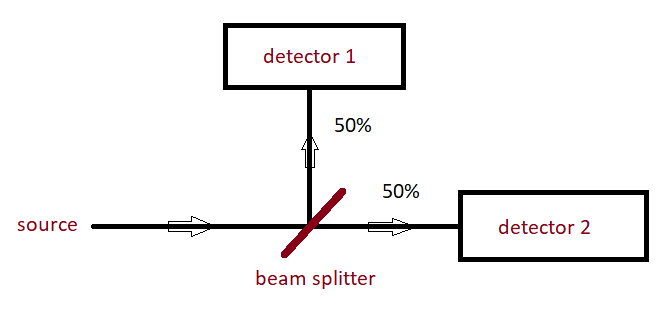
\includegraphics[height=.4\textheight]{exp1}
  \end{center}
  Suppose we have an experimental set-up consisting of a photon source, a beam splitter and a pair of photon detectors.
  What we observe is that photons hit each detector 50\% of the time. \\~\
  
  \noindent
  \textbf{The simplest explanation here is that the beam splitter has a 50\% chance to transmit or reflect each photon.}
\end{frame}

\begin{frame}[fragile]{Experiment}
  \begin{center}
      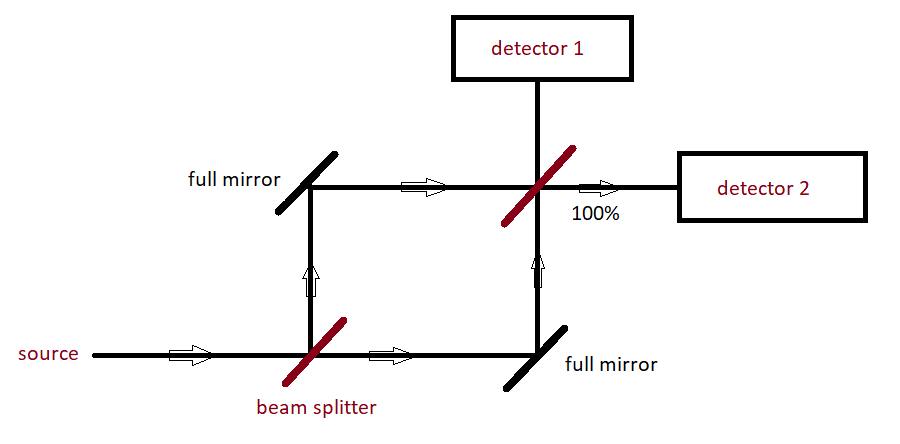
\includegraphics[height=.4\textheight]{exp2}
  \end{center}
  We modify the experiment by adding a second beam splitter and two fully reflecting mirrors.
  In this modified set-up the result is non-intuitive. The photons do not hit each detector with a 50\% chance. \\~\

  \textbf{The photons arrive at the same detector, detector 2, 100\% of the time.}

\end{frame}

\begin{frame}[fragile]{Experiment}
  \textbf{The mathematical framework of quantum physics models the experiment in a way that correctly predicts the observed outcomes.}

  FIXME
  
  The beam splitter can be model by the following operator:
  $\frac{1}{\sqrt{2}}\begin{bmatrix} 1 & i \\ i & 1 \end{bmatrix}$

  Photon state after the first beam splitter :
  $$\frac{1}{\sqrt{2}}\begin{bmatrix} 1 & i \\ i & 1 \end{bmatrix} \begin{pmatrix} 1 \\ 0 \end{pmatrix} =
  \frac{1}{\sqrt{2}} \begin{pmatrix} 1 \\ i \end{pmatrix}$$, implies proba 0.5 for path FIXME

  Photon state after the second beam splitter: $\frac{1}{\sqrt{2}}\begin{bmatrix} 1 & i \\ i & 1 \end{bmatrix}$ FIXME
\end{frame}


%-------------------------------------------------
\section{Mathematical Framework}
%-------------------------------------------------

\subsection{Hilbert space and Dirac notation}

\begin{frame}[fragile]{Hilbert space and Dirac Notation}
  The state of a n-qbit system is described by a $2^n$-dimensional vector in a finite dimensional complex vector space,
  referred as a Hilbert space $\mathcal{H}$.
  
  \begin{block}{Dirac Notation}
    Quantum computing uses the Dirac notation. This notation saves space writing sparse vector in high dimensional
    spaces. Vectors in $\mathcal{H}$ are written inside a 'ket' as follow $|v\rangle$.
  \end{block}
\end{frame}

\begin{frame}[fragile]{Dirac Notation}
 In the Dirac notation, vectors of the $2^n$ basis of an Hilbert space of dimension $n$ are labeled using binary strings of
 length n. The binary value refers to the index of the basis vector.

 Example in $\mathcal{H}$ of dimension 4:
 \begin{center}
   $\begin{pmatrix} 0 \\ 1 \\ 0 \\ 0 \end{pmatrix} = 2^{nd}$  basis vector = $0$b$01^{th}$ in binary 0-indexed =
   $|01\rangle$
 \end{center}
 
   the 4 basis vectors are therefore $∣00⟩, ∣01⟩, ∣10⟩, ∣11⟩$.
\end{frame}

\begin{frame}[fragile]{Dirac Notation}
  For instance the following Dirac notation and column vectors are equivalent:
$$\sqrt\frac{2}{3}|01\rangle + \frac{i}{\sqrt(3)}|11\rangle \Longleftrightarrow \begin{pmatrix}0 \\ \sqrt\frac{2}{3}
    \\ 0 \\ \frac{i}{\sqrt(3)} \end{pmatrix}$$
  As you can see, this notation saves space when the dimension is high and the vectors are sparse.
\end{frame}

\begin{frame}[fragile]{Dual vector and inner product}
    \begin{block}{Dual vector}
       $\langle x |$ - $x$ written inside a 'brac'
    \end{block}
  A dual vector is obtained by taking the corresponding row matrix of $x$ and then the complex conjugate of every element (Hermitean conjugate). This allows writing inner product as $\langle x | y \rangle$:
$$\langle x || y \rangle \equiv \langle x | y \rangle = \begin{pmatrix} x_1 \\ x_2 \end{pmatrix}
  \cdot \begin{pmatrix} y_1 \\ y_2 \end{pmatrix} = (x_1^* x_2^*)\begin{pmatrix} y_1 \\ y_2 \end{pmatrix} = \Sigma_i^2x_i^* y_i$$ ,
    where $c^*=a-bi$  for  $c=a+bi$
\end{frame}

\subsection{Common mathematical operators}

\begin{frame}[fragile]{Tensor product}
  \begin{block}{Tensor product}
   $|x\rangle\otimes|y\rangle$ also written $|x\rangle|y\rangle$ or $|xy\rangle$
  \end{block}
  Stitch result matrices of multiplying each element $x_i$ in x by the vector y:
$$|x\rangle\otimes|y\rangle = \begin{pmatrix} x_0 \\ x_1 \end{pmatrix} \otimes \begin{pmatrix} y_0 \\ y_1 \end{pmatrix}
  = \begin{pmatrix} x_0 y_0 \\ x_0 y_1 \\ x_1 y_0 \\ x_1 y_1 \end{pmatrix}$$, in a 2d space.
  
Example: $$\sqrt\frac{2}{3}|01\rangle + \frac{i}{\sqrt(3)}|11\rangle \Longleftrightarrow \sqrt\frac{2}{3}|0\rangle\otimes|1\rangle + \frac{i}{\sqrt(3)}|1\rangle\otimes|1\rangle$$
\end{frame}

%-------------------------------------------------
\section{Quantum Algorithm}
%-------------------------------------------------

\subsection{Shor's algorithm}

\begin{frame}[fragile]{Shor's Algorithm}
  test
\end{frame}


\subsection{Groover's algorithm}
\begin{frame}[fragile]{Groover's Algorithm}
test
\end{frame}

\section*{Bibliography}
\begin{frame}[allowframebreaks]{Bibliography}
\printbibliography
\end{frame}

\end{document}
